%\begin{evenBlock}{Gate Dribbling (10 min)}
%Set up 3 gates in a zig-zag pattern about 6 to 10 yards apart.  The gates should be about a yard wide or less depending on dribbling skill of the group.  Players start a the end line and dribble through the gates as fast as possible.  Use the same technique as the previous drill.
%\end{evenBlock}

\begin{oddBlock}{De-Acceleration Shuddle}

\begin{minipage}[t]{\linewidth}
    \centering
    
    \begin{minipage}{.2\linewidth} % Left column and width
        %\begin{figure}
            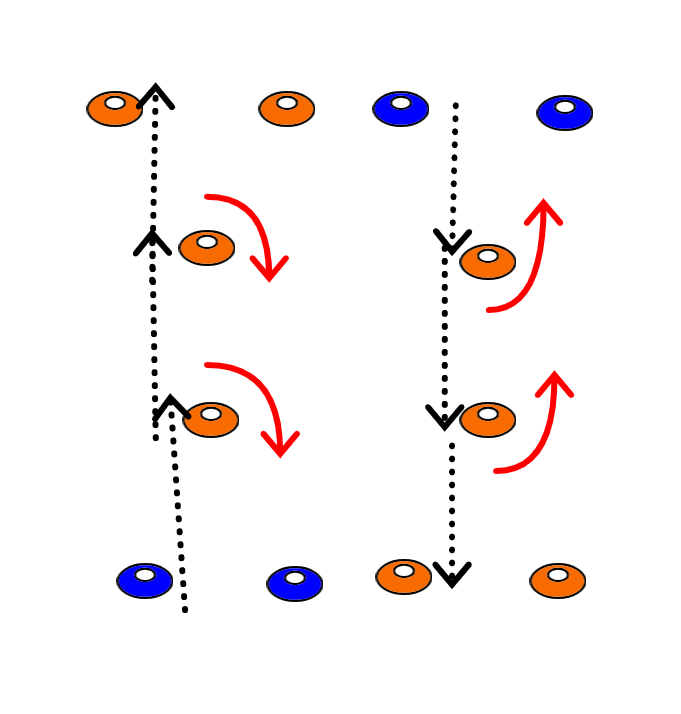
\includegraphics[width=\textwidth]{../img/Trimmed/deaccel_shuddle}
        %    \caption{Drill: 4 Person Passing}
        %\end{figure}
    \end{minipage}
    \hspace{0.05\linewidth}
    \begin{minipage}{.7\linewidth} % Left column and width
        \textbf{Drill Description:}
        This is an agility drill to practice both acceleration and de-acceleration.
        \begin{enumerate}
        \setlength{\itemsep}{0pt}
        \setlength{\parskip}{0pt}
        \setlength{\parsep}{0pt}
        \item Players start at blue gate, sprint to the left hand side of the orange cone,
        \item Shuttle around the cone using at least 6 quick toe taps.
        \item Then accelerate to the left of the next orange cone and shuttle around the cone.
        \item They finish with a full sprint through the orange gate.
        \item Return on the right set however the approach is to the right hand side of the cone.
        \item Repeat each set 4 times.
        \end{enumerate}
    \end{minipage}
\end{minipage}
    \vspace{12pt}
    
    \textbf{Coaching Points:}
    \begin{itemize}
        \setlength{\itemsep}{0pt}
        \setlength{\parskip}{0pt}
        \setlength{\parsep}{0pt}
        \item Focus on quickly getting to speed then slowing down.
        \item Focus on using small quicks touches around the cone, keeping it tight.
        \item Stay low and use your bend legs to explode away,
        \item Then compress them to slow down.
        \item Finish strong by sprinting right through the last gate, jogging back to the next blue gate.
    \end{itemize}
\end{oddBlock}